\section{« pour »}
\begin{tcolorbox}[arc=5pt, colback=white!0, colframe=orange!50!black]
\infbox{
Insertion de \textbf{« pour »}
}
\begin{center}
\tbox{
\begin{tikzpicture}
[
    level 1/.style={sibling distance=75mm, scale=1},
    level/.style={sibling distance=45mm, scale=1},
]
\node [fill=yellow, scale=1.00]
{($\underset{\text{}}{\text{pour}}$, 1)} 
;
\end{tikzpicture}
}
\end{center}

\end{tcolorbox}\section{« savoir »}
\begin{tcolorbox}[arc=5pt, colback=white!0, colframe=orange!50!black]
\infbox{
Insertion de \textbf{« savoir »}
}
\begin{center}
\tbox{
\begin{tikzpicture}
[
    level 1/.style={sibling distance=75mm, scale=1},
    level/.style={sibling distance=45mm, scale=1},
]
\node [, scale=1.00]
{($\underset{\text{}}{\text{pour}}$, 1)} 
    child {node[fill=yellow, scale=0.97]
{($\underset{\text{}}{\text{savoir}}$, 1)} 
};
\end{tikzpicture}
}
\end{center}

\end{tcolorbox}\section{« si »}
\begin{tcolorbox}[arc=5pt, colback=white!0, colframe=orange!50!black]
\infbox{
Insertion de \textbf{« si »}
}
\begin{center}
\tbox{
\begin{tikzpicture}
[
    level 1/.style={sibling distance=75mm, scale=1},
    level/.style={sibling distance=45mm, scale=1},
]
\node [, scale=1.00]
{($\underset{\text{}}{\text{pour}}$, 1)} 
    child {node[, scale=0.97]
{($\underset{\text{}}{\text{savoir}}$, 1)} 
    child {node[fill=yellow, scale=0.93]
{($\underset{\text{}}{\text{si}}$, 1)} 
}};
\end{tikzpicture}
}
\end{center}

\end{tcolorbox}\section{« un »}
\begin{tcolorbox}[arc=5pt, colback=white!0, colframe=orange!50!black]
\infbox{
Insertion de \textbf{« un »}
}
\begin{center}
\tbox{
\begin{tikzpicture}
[
    level 1/.style={sibling distance=75mm, scale=1},
    level/.style={sibling distance=45mm, scale=1},
]
\node [, scale=1.00]
{($\underset{\text{}}{\text{pour}}$, 1)} 
    child {node[, scale=0.97]
{($\underset{\text{}}{\text{savoir}}$, 1)} 
    child {node[, scale=0.93]
{($\underset{\text{}}{\text{si}}$, 1)} 
    child {node[fill=yellow, scale=0.90]
{($\underset{\text{}}{\text{un}}$, 1)} 
}}};
\end{tikzpicture}
}
\end{center}

\end{tcolorbox}\section{« mot »}
\begin{tcolorbox}[arc=5pt, colback=white!0, colframe=orange!50!black]
\infbox{
Insertion de \textbf{« mot »}
}
\begin{center}
\tbox{
\begin{tikzpicture}
[
    level 1/.style={sibling distance=75mm, scale=1},
    level/.style={sibling distance=45mm, scale=1},
]
\node [, scale=1.00]
{($\underset{\text{}}{\text{pour}}$, 1)} 
    child {node[fill=yellow, scale=0.97]
{($\underset{\text{}}{\text{mot}}$, 1)} 
}    child {node[, scale=0.97]
{($\underset{\text{}}{\text{savoir}}$, 1)} 
    child {node[, scale=0.93]
{($\underset{\text{}}{\text{si}}$, 1)} 
    child {node[, scale=0.90]
{($\underset{\text{}}{\text{un}}$, 1)} 
}}};
\end{tikzpicture}
}
\end{center}

\end{tcolorbox}\section{« est »}
\begin{tcolorbox}[arc=5pt, colback=white!0, colframe=orange!50!black]
\infbox{
Insertion de \textbf{« est »}
}
\begin{center}
\tbox{
\begin{tikzpicture}
[
    level 1/.style={sibling distance=75mm, scale=1},
    level/.style={sibling distance=45mm, scale=1},
]
\node [, scale=1.00]
{($\underset{\text{}}{\text{pour}}$, 1)} 
    child {node[, scale=0.97]
{($\underset{\text{}}{\text{mot}}$, 1)} 
    child {node[fill=yellow, scale=0.93]
{($\underset{\text{}}{\text{est}}$, 1)} 
}}    child {node[, scale=0.97]
{($\underset{\text{}}{\text{savoir}}$, 1)} 
    child {node[, scale=0.93]
{($\underset{\text{}}{\text{si}}$, 1)} 
    child {node[, scale=0.90]
{($\underset{\text{}}{\text{un}}$, 1)} 
}}};
\end{tikzpicture}
}
\end{center}

\end{tcolorbox}\section{« mal »}
\begin{tcolorbox}[arc=5pt, colback=white!0, colframe=orange!50!black]
\infbox{
Insertion de \textbf{« mal »}
}
\begin{center}
\tbox{
\begin{tikzpicture}
[
    level 1/.style={sibling distance=75mm, scale=1},
    level/.style={sibling distance=45mm, scale=1},
]
\node [, scale=1.00]
{($\underset{\text{}}{\text{pour}}$, 1)} 
    child {node[, scale=0.97]
{($\underset{\text{}}{\text{mot}}$, 1)} 
    child {node[, scale=0.93]
{($\underset{\text{}}{\text{est}}$, 1)} 
    child {node[fill=yellow, scale=0.90]
{($\underset{\text{}}{\text{mal}}$, 1)} 
}}}    child {node[, scale=0.97]
{($\underset{\text{}}{\text{savoir}}$, 1)} 
    child {node[, scale=0.93]
{($\underset{\text{}}{\text{si}}$, 1)} 
    child {node[, scale=0.90]
{($\underset{\text{}}{\text{un}}$, 1)} 
}}};
\end{tikzpicture}
}
\end{center}

\end{tcolorbox}\section{« il »}
\begin{tcolorbox}[arc=5pt, colback=white!0, colframe=orange!50!black]
\infbox{
Insertion de \textbf{« il »}
}
\begin{center}
\tbox{
\begin{tikzpicture}
[
    level 1/.style={sibling distance=75mm, scale=1},
    level/.style={sibling distance=45mm, scale=1},
]
\node [, scale=1.00]
{($\underset{\text{}}{\text{pour}}$, 1)} 
    child {node[, scale=0.97]
{($\underset{\text{}}{\text{mot}}$, 1)} 
    child {node[, scale=0.93]
{($\underset{\text{}}{\text{est}}$, 1)} 
    child {node[, scale=0.90]
{($\underset{\text{}}{\text{mal}}$, 1)} 
    child {node[fill=yellow, scale=0.87]
{($\underset{\text{}}{\text{il}}$, 1)} 
}}}}    child {node[, scale=0.97]
{($\underset{\text{}}{\text{savoir}}$, 1)} 
    child {node[, scale=0.93]
{($\underset{\text{}}{\text{si}}$, 1)} 
    child {node[, scale=0.90]
{($\underset{\text{}}{\text{un}}$, 1)} 
}}};
\end{tikzpicture}
}
\end{center}

\end{tcolorbox}\section{« suffit »}
\begin{tcolorbox}[arc=5pt, colback=white!0, colframe=orange!50!black]
\infbox{
Insertion de \textbf{« suffit »}
}
\begin{center}
\tbox{
\begin{tikzpicture}
[
    level 1/.style={sibling distance=75mm, scale=1},
    level/.style={sibling distance=45mm, scale=1},
]
\node [, scale=1.00]
{($\underset{\text{}}{\text{pour}}$, 1)} 
    child {node[, scale=0.97]
{($\underset{\text{}}{\text{mot}}$, 1)} 
    child {node[, scale=0.93]
{($\underset{\text{}}{\text{est}}$, 1)} 
    child {node[, scale=0.90]
{($\underset{\text{}}{\text{mal}}$, 1)} 
    child {node[, scale=0.87]
{($\underset{\text{}}{\text{il}}$, 1)} 
}}}}    child {node[, scale=0.97]
{($\underset{\text{}}{\text{savoir}}$, 1)} 
    child {node[, scale=0.93]
{($\underset{\text{}}{\text{si}}$, 1)} 
    child {node[, scale=0.90]
{($\underset{\text{}}{\text{un}}$, 1)} 
    child {node[fill=yellow, scale=0.87]
{($\underset{\text{}}{\text{suffit}}$, 1)} 
}}}};
\end{tikzpicture}
}
\end{center}

\end{tcolorbox}\section{« de »}
\begin{tcolorbox}[arc=5pt, colback=white!0, colframe=orange!50!black]
\infbox{
Insertion de \textbf{« de »}
}
\begin{center}
\tbox{
\begin{tikzpicture}
[
    level 1/.style={sibling distance=75mm, scale=1},
    level/.style={sibling distance=45mm, scale=1},
]
\node [, scale=1.00]
{($\underset{\text{}}{\text{pour}}$, 1)} 
    child {node[, scale=0.97]
{($\underset{\text{}}{\text{mot}}$, 1)} 
    child {node[, scale=0.93]
{($\underset{\text{}}{\text{est}}$, 1)} 
    child {node[fill=yellow, scale=0.90]
{($\underset{\text{}}{\text{de}}$, 1)} 
}    child {node[, scale=0.90]
{($\underset{\text{}}{\text{mal}}$, 1)} 
    child {node[, scale=0.87]
{($\underset{\text{}}{\text{il}}$, 1)} 
}}}}    child {node[, scale=0.97]
{($\underset{\text{}}{\text{savoir}}$, 1)} 
    child {node[, scale=0.93]
{($\underset{\text{}}{\text{si}}$, 1)} 
    child {node[, scale=0.90]
{($\underset{\text{}}{\text{un}}$, 1)} 
    child {node[, scale=0.87]
{($\underset{\text{}}{\text{suffit}}$, 1)} 
}}}};
\end{tikzpicture}
}
\end{center}

\end{tcolorbox}\section{« existe »}
\begin{tcolorbox}[arc=5pt, colback=white!0, colframe=orange!50!black]
\infbox{
Insertion de \textbf{« existe »}
}
\begin{center}
\tbox{
\begin{tikzpicture}
[
    level 1/.style={sibling distance=75mm, scale=1},
    level/.style={sibling distance=45mm, scale=1},
]
\node [, scale=1.00]
{($\underset{\text{}}{\text{pour}}$, 1)} 
    child {node[, scale=0.97]
{($\underset{\text{}}{\text{mot}}$, 1)} 
    child {node[, scale=0.93]
{($\underset{\text{}}{\text{est}}$, 1)} 
    child {node[, scale=0.90]
{($\underset{\text{}}{\text{de}}$, 1)} 
}    child {node[, scale=0.90]
{($\underset{\text{}}{\text{mal}}$, 1)} 
    child {node[, scale=0.87]
{($\underset{\text{}}{\text{il}}$, 1)} 
    child {node[fill=yellow, scale=0.83]
{($\underset{\text{}}{\text{existe}}$, 1)} 
}}}}}    child {node[, scale=0.97]
{($\underset{\text{}}{\text{savoir}}$, 1)} 
    child {node[, scale=0.93]
{($\underset{\text{}}{\text{si}}$, 1)} 
    child {node[, scale=0.90]
{($\underset{\text{}}{\text{un}}$, 1)} 
    child {node[, scale=0.87]
{($\underset{\text{}}{\text{suffit}}$, 1)} 
}}}};
\end{tikzpicture}
}
\end{center}

\end{tcolorbox}\section{« dans »}
\begin{tcolorbox}[arc=5pt, colback=white!0, colframe=orange!50!black]
\infbox{
Insertion de \textbf{« dans »}
}
\begin{center}
\tbox{
\begin{tikzpicture}
[
    level 1/.style={sibling distance=75mm, scale=1},
    level/.style={sibling distance=45mm, scale=1},
]
\node [, scale=1.00]
{($\underset{\text{}}{\text{pour}}$, 1)} 
    child {node[, scale=0.97]
{($\underset{\text{}}{\text{mot}}$, 1)} 
    child {node[, scale=0.93]
{($\underset{\text{}}{\text{est}}$, 1)} 
    child {node[, scale=0.90]
{($\underset{\text{}}{\text{de}}$, 1)} 
    child {node[fill=yellow, scale=0.87]
{($\underset{\text{}}{\text{dans}}$, 1)} 
}}    child {node[, scale=0.90]
{($\underset{\text{}}{\text{mal}}$, 1)} 
    child {node[, scale=0.87]
{($\underset{\text{}}{\text{il}}$, 1)} 
    child {node[, scale=0.83]
{($\underset{\text{}}{\text{existe}}$, 1)} 
}}}}}    child {node[, scale=0.97]
{($\underset{\text{}}{\text{savoir}}$, 1)} 
    child {node[, scale=0.93]
{($\underset{\text{}}{\text{si}}$, 1)} 
    child {node[, scale=0.90]
{($\underset{\text{}}{\text{un}}$, 1)} 
    child {node[, scale=0.87]
{($\underset{\text{}}{\text{suffit}}$, 1)} 
}}}};
\end{tikzpicture}
}
\end{center}

\end{tcolorbox}\section{« un »}
\begin{tcolorbox}[arc=5pt, colback=white!0, colframe=orange!50!black]
\infbox{
Insertion de \textbf{« un »}
}
\begin{center}
\tbox{
\begin{tikzpicture}
[
    level 1/.style={sibling distance=75mm, scale=1},
    level/.style={sibling distance=45mm, scale=1},
]
\node [, scale=1.00]
{($\underset{\text{}}{\text{pour}}$, 1)} 
    child {node[, scale=0.97]
{($\underset{\text{}}{\text{mot}}$, 1)} 
    child {node[, scale=0.93]
{($\underset{\text{}}{\text{est}}$, 1)} 
    child {node[, scale=0.90]
{($\underset{\text{}}{\text{de}}$, 1)} 
    child {node[, scale=0.87]
{($\underset{\text{}}{\text{dans}}$, 1)} 
}}    child {node[, scale=0.90]
{($\underset{\text{}}{\text{mal}}$, 1)} 
    child {node[, scale=0.87]
{($\underset{\text{}}{\text{il}}$, 1)} 
    child {node[, scale=0.83]
{($\underset{\text{}}{\text{existe}}$, 1)} 
}}}}}    child {node[, scale=0.97]
{($\underset{\text{}}{\text{savoir}}$, 1)} 
    child {node[, scale=0.93]
{($\underset{\text{}}{\text{si}}$, 1)} 
    child {node[fill=yellow, scale=0.90]
{($\underset{\text{}}{\text{un}}$, 2)} 
    child {node[, scale=0.87]
{($\underset{\text{}}{\text{suffit}}$, 1)} 
}}}};
\end{tikzpicture}
}
\end{center}

\end{tcolorbox}
\section{« dictionnaire »}
\begin{tcolorbox}[arc=5pt, colback=white!0, colframe=orange!50!black]
\infbox{
Insertion de \textbf{« dictionnaire »}
}
\begin{center}
\tbox{
\begin{tikzpicture}
[
    level 1/.style={sibling distance=75mm, scale=1},
    level/.style={sibling distance=45mm, scale=1},
]
\node [, scale=1.00]
{($\underset{\text{si}}{\text{un}}$, 2)} 
    child {node[, scale=0.97]
{($\underset{\text{}}{\text{mot}}$, 1)} 
    child {node[, scale=0.93]
{($\underset{\text{}}{\text{est}}$, 1)} 
    child {node[, scale=0.90]
{($\underset{\text{}}{\text{de}}$, 1)} 
    child {node[, scale=0.87]
{($\underset{\text{}}{\text{dans}}$, 1)} 
}    child {node[fill=yellow, scale=0.87]
{($\underset{\text{}}{\text{dictionnaire}}$, 1)} 
}}    child {node[, scale=0.90]
{($\underset{\text{}}{\text{mal}}$, 1)} 
    child {node[, scale=0.87]
{($\underset{\text{}}{\text{il}}$, 1)} 
    child {node[, scale=0.83]
{($\underset{\text{}}{\text{existe}}$, 1)} 
}}}}}    child {node[, scale=0.97]
{($\underset{\text{un}}{\text{pour}}$, 1)} 
    child {node[, scale=0.93]
{($\underset{\text{un}}{\text{savoir}}$, 1)} 
    child {node[, scale=0.90]
{($\underset{\text{un}}{\text{si}}$, 1)} 
    child {node[, scale=0.87]
{($\underset{\text{}}{\text{suffit}}$, 1)} 
}}}};
\end{tikzpicture}
}
\end{center}

\end{tcolorbox}\section{« par »}
\begin{tcolorbox}[arc=5pt, colback=white!0, colframe=orange!50!black]
\infbox{
Insertion de \textbf{« par »}
}
\begin{center}
\tbox{
\begin{tikzpicture}
[
    level 1/.style={sibling distance=75mm, scale=1},
    level/.style={sibling distance=45mm, scale=1},
]
\node [, scale=1.00]
{($\underset{\text{si}}{\text{un}}$, 2)} 
    child {node[, scale=0.97]
{($\underset{\text{}}{\text{mot}}$, 1)} 
    child {node[, scale=0.93]
{($\underset{\text{}}{\text{est}}$, 1)} 
    child {node[, scale=0.90]
{($\underset{\text{}}{\text{de}}$, 1)} 
    child {node[, scale=0.87]
{($\underset{\text{}}{\text{dans}}$, 1)} 
}    child {node[, scale=0.87]
{($\underset{\text{}}{\text{dictionnaire}}$, 1)} 
}}    child {node[, scale=0.90]
{($\underset{\text{}}{\text{mal}}$, 1)} 
    child {node[, scale=0.87]
{($\underset{\text{}}{\text{il}}$, 1)} 
    child {node[, scale=0.83]
{($\underset{\text{}}{\text{existe}}$, 1)} 
}}}}    child {node[fill=yellow, scale=0.93]
{($\underset{\text{}}{\text{par}}$, 1)} 
}}    child {node[, scale=0.97]
{($\underset{\text{un}}{\text{pour}}$, 1)} 
    child {node[, scale=0.93]
{($\underset{\text{un}}{\text{savoir}}$, 1)} 
    child {node[, scale=0.90]
{($\underset{\text{un}}{\text{si}}$, 1)} 
    child {node[, scale=0.87]
{($\underset{\text{}}{\text{suffit}}$, 1)} 
}}}};
\end{tikzpicture}
}
\end{center}

\end{tcolorbox}\section{« contre »}
\begin{tcolorbox}[arc=5pt, colback=white!0, colframe=orange!50!black]
\infbox{
Insertion de \textbf{« contre »}
}
\begin{center}
\tbox{
\begin{tikzpicture}
[
    level 1/.style={sibling distance=75mm, scale=1},
    level/.style={sibling distance=45mm, scale=1},
]
\node [, scale=1.00]
{($\underset{\text{si}}{\text{un}}$, 2)} 
    child {node[, scale=0.97]
{($\underset{\text{}}{\text{mot}}$, 1)} 
    child {node[, scale=0.93]
{($\underset{\text{}}{\text{est}}$, 1)} 
    child {node[, scale=0.90]
{($\underset{\text{}}{\text{de}}$, 1)} 
    child {node[, scale=0.87]
{($\underset{\text{}}{\text{dans}}$, 1)} 
    child {node[fill=yellow, scale=0.83]
{($\underset{\text{}}{\text{contre}}$, 1)} 
}}    child {node[, scale=0.87]
{($\underset{\text{}}{\text{dictionnaire}}$, 1)} 
}}    child {node[, scale=0.90]
{($\underset{\text{}}{\text{mal}}$, 1)} 
    child {node[, scale=0.87]
{($\underset{\text{}}{\text{il}}$, 1)} 
    child {node[, scale=0.83]
{($\underset{\text{}}{\text{existe}}$, 1)} 
}}}}    child {node[, scale=0.93]
{($\underset{\text{}}{\text{par}}$, 1)} 
}}    child {node[, scale=0.97]
{($\underset{\text{un}}{\text{pour}}$, 1)} 
    child {node[, scale=0.93]
{($\underset{\text{un}}{\text{savoir}}$, 1)} 
    child {node[, scale=0.90]
{($\underset{\text{un}}{\text{si}}$, 1)} 
    child {node[, scale=0.87]
{($\underset{\text{}}{\text{suffit}}$, 1)} 
}}}};
\end{tikzpicture}
}
\end{center}

\end{tcolorbox}\section{« pour »}
\begin{tcolorbox}[arc=5pt, colback=white!0, colframe=orange!50!black]
\infbox{
Insertion de \textbf{« pour »}
}
\begin{center}
\tbox{
\begin{tikzpicture}
[
    level 1/.style={sibling distance=75mm, scale=1},
    level/.style={sibling distance=45mm, scale=1},
]
\node [, scale=1.00]
{($\underset{\text{si}}{\text{un}}$, 2)} 
    child {node[, scale=0.97]
{($\underset{\text{}}{\text{mot}}$, 1)} 
    child {node[, scale=0.93]
{($\underset{\text{}}{\text{est}}$, 1)} 
    child {node[, scale=0.90]
{($\underset{\text{}}{\text{de}}$, 1)} 
    child {node[, scale=0.87]
{($\underset{\text{}}{\text{dans}}$, 1)} 
    child {node[, scale=0.83]
{($\underset{\text{}}{\text{contre}}$, 1)} 
}}    child {node[, scale=0.87]
{($\underset{\text{}}{\text{dictionnaire}}$, 1)} 
}}    child {node[, scale=0.90]
{($\underset{\text{}}{\text{mal}}$, 1)} 
    child {node[, scale=0.87]
{($\underset{\text{}}{\text{il}}$, 1)} 
    child {node[, scale=0.83]
{($\underset{\text{}}{\text{existe}}$, 1)} 
}}}}    child {node[, scale=0.93]
{($\underset{\text{}}{\text{par}}$, 1)} 
    child {node[fill=yellow, scale=0.90]
{($\underset{\text{}}{\text{pour}}$, 1)} 
}}}    child {node[fill=yellow, scale=0.97]
{($\underset{\text{un}}{\text{pour}}$, 1)} 
    child {node[, scale=0.93]
{($\underset{\text{un}}{\text{savoir}}$, 1)} 
    child {node[, scale=0.90]
{($\underset{\text{un}}{\text{si}}$, 1)} 
    child {node[, scale=0.87]
{($\underset{\text{}}{\text{suffit}}$, 1)} 
}}}};
\end{tikzpicture}
}
\end{center}

\end{tcolorbox}\section{« une »}
\begin{tcolorbox}[arc=5pt, colback=white!0, colframe=orange!50!black]
\infbox{
Insertion de \textbf{« une »}
}
\begin{center}
\tbox{
\begin{tikzpicture}
[
    level 1/.style={sibling distance=75mm, scale=1},
    level/.style={sibling distance=45mm, scale=1},
]
\node [, scale=1.00]
{($\underset{\text{si}}{\text{un}}$, 2)} 
    child {node[, scale=0.97]
{($\underset{\text{}}{\text{mot}}$, 1)} 
    child {node[, scale=0.93]
{($\underset{\text{}}{\text{est}}$, 1)} 
    child {node[, scale=0.90]
{($\underset{\text{}}{\text{de}}$, 1)} 
    child {node[, scale=0.87]
{($\underset{\text{}}{\text{dans}}$, 1)} 
    child {node[, scale=0.83]
{($\underset{\text{}}{\text{contre}}$, 1)} 
}}    child {node[, scale=0.87]
{($\underset{\text{}}{\text{dictionnaire}}$, 1)} 
}}    child {node[, scale=0.90]
{($\underset{\text{}}{\text{mal}}$, 1)} 
    child {node[, scale=0.87]
{($\underset{\text{}}{\text{il}}$, 1)} 
    child {node[, scale=0.83]
{($\underset{\text{}}{\text{existe}}$, 1)} 
}}}}    child {node[, scale=0.93]
{($\underset{\text{}}{\text{par}}$, 1)} 
    child {node[, scale=0.90]
{($\underset{\text{}}{\text{pour}}$, 1)} 
}}}    child {node[, scale=0.97]
{($\underset{\text{un}}{\text{pour}}$, 1)} 
    child {node[, scale=0.93]
{($\underset{\text{un}}{\text{savoir}}$, 1)} 
    child {node[, scale=0.90]
{($\underset{\text{un}}{\text{si}}$, 1)} 
    child {node[, scale=0.87]
{($\underset{\text{}}{\text{suffit}}$, 1)} 
}    child {node[fill=yellow, scale=0.87]
{($\underset{\text{}}{\text{une}}$, 1)} 
}}}};
\end{tikzpicture}
}
\end{center}

\end{tcolorbox}\section{« correction »}
\begin{tcolorbox}[arc=5pt, colback=white!0, colframe=orange!50!black]
\infbox{
Insertion de \textbf{« correction »}
}
\begin{center}
\tbox{
\begin{tikzpicture}
[
    level 1/.style={sibling distance=75mm, scale=1},
    level/.style={sibling distance=45mm, scale=1},
]
\node [, scale=1.00]
{($\underset{\text{si}}{\text{un}}$, 2)} 
    child {node[, scale=0.97]
{($\underset{\text{}}{\text{mot}}$, 1)} 
    child {node[, scale=0.93]
{($\underset{\text{}}{\text{est}}$, 1)} 
    child {node[, scale=0.90]
{($\underset{\text{}}{\text{de}}$, 1)} 
    child {node[, scale=0.87]
{($\underset{\text{}}{\text{dans}}$, 1)} 
    child {node[, scale=0.83]
{($\underset{\text{}}{\text{contre}}$, 1)} 
    child {node[fill=yellow, scale=0.80]
{($\underset{\text{}}{\text{correction}}$, 1)} 
}}}    child {node[, scale=0.87]
{($\underset{\text{}}{\text{dictionnaire}}$, 1)} 
}}    child {node[, scale=0.90]
{($\underset{\text{}}{\text{mal}}$, 1)} 
    child {node[, scale=0.87]
{($\underset{\text{}}{\text{il}}$, 1)} 
    child {node[, scale=0.83]
{($\underset{\text{}}{\text{existe}}$, 1)} 
}}}}    child {node[, scale=0.93]
{($\underset{\text{}}{\text{par}}$, 1)} 
    child {node[, scale=0.90]
{($\underset{\text{}}{\text{pour}}$, 1)} 
}}}    child {node[, scale=0.97]
{($\underset{\text{un}}{\text{pour}}$, 1)} 
    child {node[, scale=0.93]
{($\underset{\text{un}}{\text{savoir}}$, 1)} 
    child {node[, scale=0.90]
{($\underset{\text{un}}{\text{si}}$, 1)} 
    child {node[, scale=0.87]
{($\underset{\text{}}{\text{suffit}}$, 1)} 
}    child {node[, scale=0.87]
{($\underset{\text{}}{\text{une}}$, 1)} 
}}}};
\end{tikzpicture}
}
\end{center}

\end{tcolorbox}\section{« orthographique »}
\begin{tcolorbox}[arc=5pt, colback=white!0, colframe=orange!50!black]
\infbox{
Insertion de \textbf{« orthographique »}
}
\begin{center}
\tbox{
\begin{tikzpicture}
[
    level 1/.style={sibling distance=75mm, scale=1},
    level/.style={sibling distance=45mm, scale=1},
]
\node [, scale=1.00]
{($\underset{\text{si}}{\text{un}}$, 2)} 
    child {node[, scale=0.97]
{($\underset{\text{}}{\text{mot}}$, 1)} 
    child {node[, scale=0.93]
{($\underset{\text{}}{\text{est}}$, 1)} 
    child {node[, scale=0.90]
{($\underset{\text{}}{\text{de}}$, 1)} 
    child {node[, scale=0.87]
{($\underset{\text{}}{\text{dans}}$, 1)} 
    child {node[, scale=0.83]
{($\underset{\text{}}{\text{contre}}$, 1)} 
    child {node[, scale=0.80]
{($\underset{\text{}}{\text{correction}}$, 1)} 
}}}    child {node[, scale=0.87]
{($\underset{\text{}}{\text{dictionnaire}}$, 1)} 
}}    child {node[, scale=0.90]
{($\underset{\text{}}{\text{mal}}$, 1)} 
    child {node[, scale=0.87]
{($\underset{\text{}}{\text{il}}$, 1)} 
    child {node[, scale=0.83]
{($\underset{\text{}}{\text{existe}}$, 1)} 
}}}}    child {node[, scale=0.93]
{($\underset{\text{}}{\text{par}}$, 1)} 
    child {node[fill=yellow, scale=0.90]
{($\underset{\text{}}{\text{orthographique}}$, 1)} 
}    child {node[, scale=0.90]
{($\underset{\text{}}{\text{pour}}$, 1)} 
}}}    child {node[, scale=0.97]
{($\underset{\text{un}}{\text{pour}}$, 1)} 
    child {node[, scale=0.93]
{($\underset{\text{un}}{\text{savoir}}$, 1)} 
    child {node[, scale=0.90]
{($\underset{\text{un}}{\text{si}}$, 1)} 
    child {node[, scale=0.87]
{($\underset{\text{}}{\text{suffit}}$, 1)} 
}    child {node[, scale=0.87]
{($\underset{\text{}}{\text{une}}$, 1)} 
}}}};
\end{tikzpicture}
}
\end{center}

\end{tcolorbox}\section{« il »}
\begin{tcolorbox}[arc=5pt, colback=white!0, colframe=orange!50!black]
\infbox{
Insertion de \textbf{« il »}
}
\begin{center}
\tbox{
\begin{tikzpicture}
[
    level 1/.style={sibling distance=75mm, scale=1},
    level/.style={sibling distance=45mm, scale=1},
]
\node [, scale=1.00]
{($\underset{\text{si}}{\text{un}}$, 2)} 
    child {node[, scale=0.97]
{($\underset{\text{}}{\text{mot}}$, 1)} 
    child {node[, scale=0.93]
{($\underset{\text{}}{\text{est}}$, 1)} 
    child {node[, scale=0.90]
{($\underset{\text{}}{\text{de}}$, 1)} 
    child {node[, scale=0.87]
{($\underset{\text{}}{\text{dans}}$, 1)} 
    child {node[, scale=0.83]
{($\underset{\text{}}{\text{contre}}$, 1)} 
    child {node[, scale=0.80]
{($\underset{\text{}}{\text{correction}}$, 1)} 
}}}    child {node[, scale=0.87]
{($\underset{\text{}}{\text{dictionnaire}}$, 1)} 
}}    child {node[, scale=0.90]
{($\underset{\text{}}{\text{mal}}$, 1)} 
    child {node[fill=yellow, scale=0.87]
{($\underset{\text{}}{\text{il}}$, 2)} 
    child {node[, scale=0.83]
{($\underset{\text{}}{\text{existe}}$, 1)} 
}}}}    child {node[, scale=0.93]
{($\underset{\text{}}{\text{par}}$, 1)} 
    child {node[, scale=0.90]
{($\underset{\text{}}{\text{orthographique}}$, 1)} 
}    child {node[, scale=0.90]
{($\underset{\text{}}{\text{pour}}$, 1)} 
}}}    child {node[, scale=0.97]
{($\underset{\text{un}}{\text{pour}}$, 1)} 
    child {node[, scale=0.93]
{($\underset{\text{un}}{\text{savoir}}$, 1)} 
    child {node[, scale=0.90]
{($\underset{\text{un}}{\text{si}}$, 1)} 
    child {node[, scale=0.87]
{($\underset{\text{}}{\text{suffit}}$, 1)} 
}    child {node[, scale=0.87]
{($\underset{\text{}}{\text{une}}$, 1)} 
}}}};
\end{tikzpicture}
}
\end{center}

\end{tcolorbox}
\section{« faut »}
\begin{tcolorbox}[arc=5pt, colback=white!0, colframe=orange!50!black]
\infbox{
Insertion de \textbf{« faut »}
}
\begin{center}
\tbox{
\begin{tikzpicture}
[
    level 1/.style={sibling distance=75mm, scale=1},
    level/.style={sibling distance=45mm, scale=1},
]
\node [, scale=1.00]
{($\underset{\text{si}}{\text{un}}$, 2)} 
    child {node[, scale=0.97]
{($\underset{\text{mal}}{\text{il}}$, 2)} 
    child {node[, scale=0.93]
{($\underset{\text{il}}{\text{mot}}$, 1)} 
    child {node[, scale=0.90]
{($\underset{\text{}}{\text{de}}$, 1)} 
    child {node[, scale=0.87]
{($\underset{\text{}}{\text{dans}}$, 1)} 
    child {node[, scale=0.83]
{($\underset{\text{}}{\text{contre}}$, 1)} 
    child {node[, scale=0.80]
{($\underset{\text{}}{\text{correction}}$, 1)} 
}}}    child {node[, scale=0.87]
{($\underset{\text{}}{\text{dictionnaire}}$, 1)} 
    child {node[fill=yellow, scale=0.83]
{($\underset{\text{}}{\text{faut}}$, 1)} 
}}}    child {node[, scale=0.90]
{($\underset{\text{il}}{\text{est}}$, 1)} 
    child {node[, scale=0.87]
{($\underset{\text{il}}{\text{mal}}$, 1)} 
    child {node[, scale=0.83]
{($\underset{\text{}}{\text{existe}}$, 1)} 
}}}}    child {node[, scale=0.93]
{($\underset{\text{}}{\text{par}}$, 1)} 
    child {node[, scale=0.90]
{($\underset{\text{}}{\text{orthographique}}$, 1)} 
}    child {node[, scale=0.90]
{($\underset{\text{}}{\text{pour}}$, 1)} 
}}}    child {node[, scale=0.97]
{($\underset{\text{un}}{\text{pour}}$, 1)} 
    child {node[, scale=0.93]
{($\underset{\text{un}}{\text{savoir}}$, 1)} 
    child {node[, scale=0.90]
{($\underset{\text{un}}{\text{si}}$, 1)} 
    child {node[, scale=0.87]
{($\underset{\text{}}{\text{suffit}}$, 1)} 
}    child {node[, scale=0.87]
{($\underset{\text{}}{\text{une}}$, 1)} 
}}}};
\end{tikzpicture}
}
\end{center}

\end{tcolorbox}\section{« proposer »}
\begin{tcolorbox}[arc=5pt, colback=white!0, colframe=orange!50!black]
\infbox{
Insertion de \textbf{« proposer »}
}
\begin{center}
\tbox{
\begin{tikzpicture}
[
    level 1/.style={sibling distance=75mm, scale=1},
    level/.style={sibling distance=45mm, scale=1},
]
\node [, scale=1.00]
{($\underset{\text{si}}{\text{un}}$, 2)} 
    child {node[, scale=0.97]
{($\underset{\text{mal}}{\text{il}}$, 2)} 
    child {node[, scale=0.93]
{($\underset{\text{il}}{\text{mot}}$, 1)} 
    child {node[, scale=0.90]
{($\underset{\text{}}{\text{de}}$, 1)} 
    child {node[, scale=0.87]
{($\underset{\text{}}{\text{dans}}$, 1)} 
    child {node[, scale=0.83]
{($\underset{\text{}}{\text{contre}}$, 1)} 
    child {node[, scale=0.80]
{($\underset{\text{}}{\text{correction}}$, 1)} 
}}}    child {node[, scale=0.87]
{($\underset{\text{}}{\text{dictionnaire}}$, 1)} 
    child {node[, scale=0.83]
{($\underset{\text{}}{\text{faut}}$, 1)} 
}}}    child {node[, scale=0.90]
{($\underset{\text{il}}{\text{est}}$, 1)} 
    child {node[, scale=0.87]
{($\underset{\text{il}}{\text{mal}}$, 1)} 
    child {node[, scale=0.83]
{($\underset{\text{}}{\text{existe}}$, 1)} 
}}}}    child {node[, scale=0.93]
{($\underset{\text{}}{\text{par}}$, 1)} 
    child {node[, scale=0.90]
{($\underset{\text{}}{\text{orthographique}}$, 1)} 
}    child {node[, scale=0.90]
{($\underset{\text{}}{\text{pour}}$, 1)} 
    child {node[fill=yellow, scale=0.87]
{($\underset{\text{}}{\text{proposer}}$, 1)} 
}}}}    child {node[, scale=0.97]
{($\underset{\text{un}}{\text{pour}}$, 1)} 
    child {node[, scale=0.93]
{($\underset{\text{un}}{\text{savoir}}$, 1)} 
    child {node[, scale=0.90]
{($\underset{\text{un}}{\text{si}}$, 1)} 
    child {node[, scale=0.87]
{($\underset{\text{}}{\text{suffit}}$, 1)} 
}    child {node[, scale=0.87]
{($\underset{\text{}}{\text{une}}$, 1)} 
}}}};
\end{tikzpicture}
}
\end{center}

\end{tcolorbox}\section{« un »}
\begin{tcolorbox}[arc=5pt, colback=white!0, colframe=orange!50!black]
\infbox{
Insertion de \textbf{« un »}
}
\begin{center}
\tbox{
\begin{tikzpicture}
[
    level 1/.style={sibling distance=75mm, scale=1},
    level/.style={sibling distance=45mm, scale=1},
]
\node [fill=yellow, scale=1.00]
{($\underset{\text{si}}{\text{un}}$, 3)} 
    child {node[, scale=0.97]
{($\underset{\text{mal}}{\text{il}}$, 2)} 
    child {node[, scale=0.93]
{($\underset{\text{il}}{\text{mot}}$, 1)} 
    child {node[, scale=0.90]
{($\underset{\text{}}{\text{de}}$, 1)} 
    child {node[, scale=0.87]
{($\underset{\text{}}{\text{dans}}$, 1)} 
    child {node[, scale=0.83]
{($\underset{\text{}}{\text{contre}}$, 1)} 
    child {node[, scale=0.80]
{($\underset{\text{}}{\text{correction}}$, 1)} 
}}}    child {node[, scale=0.87]
{($\underset{\text{}}{\text{dictionnaire}}$, 1)} 
    child {node[, scale=0.83]
{($\underset{\text{}}{\text{faut}}$, 1)} 
}}}    child {node[, scale=0.90]
{($\underset{\text{il}}{\text{est}}$, 1)} 
    child {node[, scale=0.87]
{($\underset{\text{il}}{\text{mal}}$, 1)} 
    child {node[, scale=0.83]
{($\underset{\text{}}{\text{existe}}$, 1)} 
}}}}    child {node[, scale=0.93]
{($\underset{\text{}}{\text{par}}$, 1)} 
    child {node[, scale=0.90]
{($\underset{\text{}}{\text{orthographique}}$, 1)} 
}    child {node[, scale=0.90]
{($\underset{\text{}}{\text{pour}}$, 1)} 
    child {node[, scale=0.87]
{($\underset{\text{}}{\text{proposer}}$, 1)} 
}}}}    child {node[, scale=0.97]
{($\underset{\text{un}}{\text{pour}}$, 1)} 
    child {node[, scale=0.93]
{($\underset{\text{un}}{\text{savoir}}$, 1)} 
    child {node[, scale=0.90]
{($\underset{\text{un}}{\text{si}}$, 1)} 
    child {node[, scale=0.87]
{($\underset{\text{}}{\text{suffit}}$, 1)} 
}    child {node[, scale=0.87]
{($\underset{\text{}}{\text{une}}$, 1)} 
}}}};
\end{tikzpicture}
}
\end{center}

\end{tcolorbox}
\section{« mot »}
\begin{tcolorbox}[arc=5pt, colback=white!0, colframe=orange!50!black]
\infbox{
Insertion de \textbf{« mot »}
}
\begin{center}
\tbox{
\begin{tikzpicture}
[
    level 1/.style={sibling distance=75mm, scale=1},
    level/.style={sibling distance=45mm, scale=1},
]
\node [, scale=1.00]
{($\underset{\text{si}}{\text{un}}$, 3)} 
    child {node[, scale=0.97]
{($\underset{\text{mal}}{\text{il}}$, 2)} 
    child {node[fill=yellow, scale=0.93]
{($\underset{\text{il}}{\text{mot}}$, 1)} 
    child {node[, scale=0.90]
{($\underset{\text{}}{\text{de}}$, 1)} 
    child {node[, scale=0.87]
{($\underset{\text{}}{\text{dans}}$, 1)} 
    child {node[, scale=0.83]
{($\underset{\text{}}{\text{contre}}$, 1)} 
    child {node[, scale=0.80]
{($\underset{\text{}}{\text{correction}}$, 1)} 
}}}    child {node[, scale=0.87]
{($\underset{\text{}}{\text{dictionnaire}}$, 1)} 
    child {node[, scale=0.83]
{($\underset{\text{}}{\text{faut}}$, 1)} 
}}}    child {node[, scale=0.90]
{($\underset{\text{il}}{\text{est}}$, 1)} 
    child {node[, scale=0.87]
{($\underset{\text{il}}{\text{mal}}$, 1)} 
    child {node[, scale=0.83]
{($\underset{\text{}}{\text{existe}}$, 1)} 
}}}}    child {node[, scale=0.93]
{($\underset{\text{}}{\text{par}}$, 1)} 
    child {node[, scale=0.90]
{($\underset{\text{}}{\text{orthographique}}$, 1)} 
    child {node[fill=yellow, scale=0.87]
{($\underset{\text{}}{\text{mot}}$, 1)} 
}}    child {node[, scale=0.90]
{($\underset{\text{}}{\text{pour}}$, 1)} 
    child {node[, scale=0.87]
{($\underset{\text{}}{\text{proposer}}$, 1)} 
}}}}    child {node[, scale=0.97]
{($\underset{\text{un}}{\text{pour}}$, 1)} 
    child {node[, scale=0.93]
{($\underset{\text{un}}{\text{savoir}}$, 1)} 
    child {node[, scale=0.90]
{($\underset{\text{un}}{\text{si}}$, 1)} 
    child {node[, scale=0.87]
{($\underset{\text{}}{\text{suffit}}$, 1)} 
}    child {node[, scale=0.87]
{($\underset{\text{}}{\text{une}}$, 1)} 
}}}};
\end{tikzpicture}
}
\end{center}

\end{tcolorbox}\section{« pour »}
\begin{tcolorbox}[arc=5pt, colback=white!0, colframe=orange!50!black]
\infbox{
Insertion de \textbf{« pour »}
}
\begin{center}
\tbox{
\begin{tikzpicture}
[
    level 1/.style={sibling distance=75mm, scale=1},
    level/.style={sibling distance=45mm, scale=1},
]
\node [, scale=1.00]
{($\underset{\text{si}}{\text{un}}$, 3)} 
    child {node[, scale=0.97]
{($\underset{\text{mal}}{\text{il}}$, 2)} 
    child {node[, scale=0.93]
{($\underset{\text{il}}{\text{mot}}$, 1)} 
    child {node[, scale=0.90]
{($\underset{\text{}}{\text{de}}$, 1)} 
    child {node[, scale=0.87]
{($\underset{\text{}}{\text{dans}}$, 1)} 
    child {node[, scale=0.83]
{($\underset{\text{}}{\text{contre}}$, 1)} 
    child {node[, scale=0.80]
{($\underset{\text{}}{\text{correction}}$, 1)} 
}}}    child {node[, scale=0.87]
{($\underset{\text{}}{\text{dictionnaire}}$, 1)} 
    child {node[, scale=0.83]
{($\underset{\text{}}{\text{faut}}$, 1)} 
}}}    child {node[, scale=0.90]
{($\underset{\text{il}}{\text{est}}$, 1)} 
    child {node[, scale=0.87]
{($\underset{\text{il}}{\text{mal}}$, 1)} 
    child {node[, scale=0.83]
{($\underset{\text{}}{\text{existe}}$, 1)} 
}}}}    child {node[, scale=0.93]
{($\underset{\text{}}{\text{par}}$, 1)} 
    child {node[, scale=0.90]
{($\underset{\text{}}{\text{orthographique}}$, 1)} 
    child {node[, scale=0.87]
{($\underset{\text{}}{\text{mot}}$, 1)} 
}}    child {node[fill=yellow, scale=0.90]
{($\underset{\text{}}{\text{pour}}$, 2)} 
    child {node[, scale=0.87]
{($\underset{\text{}}{\text{proposer}}$, 1)} 
}}}}    child {node[fill=yellow, scale=0.97]
{($\underset{\text{un}}{\text{pour}}$, 1)} 
    child {node[, scale=0.93]
{($\underset{\text{un}}{\text{savoir}}$, 1)} 
    child {node[, scale=0.90]
{($\underset{\text{un}}{\text{si}}$, 1)} 
    child {node[, scale=0.87]
{($\underset{\text{}}{\text{suffit}}$, 1)} 
}    child {node[, scale=0.87]
{($\underset{\text{}}{\text{une}}$, 1)} 
}}}};
\end{tikzpicture}
}
\end{center}

\end{tcolorbox}
\section{« cela »}
\begin{tcolorbox}[arc=5pt, colback=white!0, colframe=orange!50!black]
\infbox{
Insertion de \textbf{« cela »}
}
\begin{center}
\tbox{
\begin{tikzpicture}
[
    level 1/.style={sibling distance=75mm, scale=1},
    level/.style={sibling distance=45mm, scale=1},
]
\node [, scale=1.00]
{($\underset{\text{si}}{\text{un}}$, 3)} 
    child {node[, scale=0.97]
{($\underset{\text{mal}}{\text{il}}$, 2)} 
    child {node[, scale=0.93]
{($\underset{\text{il}}{\text{mot}}$, 1)} 
    child {node[, scale=0.90]
{($\underset{\text{}}{\text{de}}$, 1)} 
    child {node[, scale=0.87]
{($\underset{\text{}}{\text{dans}}$, 1)} 
    child {node[, scale=0.83]
{($\underset{\text{}}{\text{contre}}$, 1)} 
    child {node[fill=yellow, scale=0.80]
{($\underset{\text{}}{\text{cela}}$, 1)} 
}    child {node[, scale=0.80]
{($\underset{\text{}}{\text{correction}}$, 1)} 
}}}    child {node[, scale=0.87]
{($\underset{\text{}}{\text{dictionnaire}}$, 1)} 
    child {node[, scale=0.83]
{($\underset{\text{}}{\text{faut}}$, 1)} 
}}}    child {node[, scale=0.90]
{($\underset{\text{il}}{\text{est}}$, 1)} 
    child {node[, scale=0.87]
{($\underset{\text{il}}{\text{mal}}$, 1)} 
    child {node[, scale=0.83]
{($\underset{\text{}}{\text{existe}}$, 1)} 
}}}}    child {node[, scale=0.93]
{($\underset{\text{par}}{\text{pour}}$, 2)} 
    child {node[, scale=0.90]
{($\underset{\text{}}{\text{orthographique}}$, 1)} 
    child {node[, scale=0.87]
{($\underset{\text{}}{\text{mot}}$, 1)} 
}}    child {node[, scale=0.90]
{($\underset{\text{pour}}{\text{par}}$, 1)} 
    child {node[, scale=0.87]
{($\underset{\text{}}{\text{proposer}}$, 1)} 
}}}}    child {node[, scale=0.97]
{($\underset{\text{un}}{\text{pour}}$, 1)} 
    child {node[, scale=0.93]
{($\underset{\text{un}}{\text{savoir}}$, 1)} 
    child {node[, scale=0.90]
{($\underset{\text{un}}{\text{si}}$, 1)} 
    child {node[, scale=0.87]
{($\underset{\text{}}{\text{suffit}}$, 1)} 
}    child {node[, scale=0.87]
{($\underset{\text{}}{\text{une}}$, 1)} 
}}}};
\end{tikzpicture}
}
\end{center}

\end{tcolorbox}\section{« il »}
\begin{tcolorbox}[arc=5pt, colback=white!0, colframe=orange!50!black]
\infbox{
Insertion de \textbf{« il »}
}
\begin{center}
\tbox{
\begin{tikzpicture}
[
    level 1/.style={sibling distance=75mm, scale=1},
    level/.style={sibling distance=45mm, scale=1},
]
\node [, scale=1.00]
{($\underset{\text{si}}{\text{un}}$, 3)} 
    child {node[fill=yellow, scale=0.97]
{($\underset{\text{mal}}{\text{il}}$, 3)} 
    child {node[, scale=0.93]
{($\underset{\text{il}}{\text{mot}}$, 1)} 
    child {node[, scale=0.90]
{($\underset{\text{}}{\text{de}}$, 1)} 
    child {node[, scale=0.87]
{($\underset{\text{}}{\text{dans}}$, 1)} 
    child {node[, scale=0.83]
{($\underset{\text{}}{\text{contre}}$, 1)} 
    child {node[, scale=0.80]
{($\underset{\text{}}{\text{cela}}$, 1)} 
}    child {node[, scale=0.80]
{($\underset{\text{}}{\text{correction}}$, 1)} 
}}}    child {node[, scale=0.87]
{($\underset{\text{}}{\text{dictionnaire}}$, 1)} 
    child {node[, scale=0.83]
{($\underset{\text{}}{\text{faut}}$, 1)} 
}}}    child {node[, scale=0.90]
{($\underset{\text{il}}{\text{est}}$, 1)} 
    child {node[, scale=0.87]
{($\underset{\text{il}}{\text{mal}}$, 1)} 
    child {node[, scale=0.83]
{($\underset{\text{}}{\text{existe}}$, 1)} 
}}}}    child {node[, scale=0.93]
{($\underset{\text{par}}{\text{pour}}$, 2)} 
    child {node[, scale=0.90]
{($\underset{\text{}}{\text{orthographique}}$, 1)} 
    child {node[, scale=0.87]
{($\underset{\text{}}{\text{mot}}$, 1)} 
}}    child {node[, scale=0.90]
{($\underset{\text{pour}}{\text{par}}$, 1)} 
    child {node[, scale=0.87]
{($\underset{\text{}}{\text{proposer}}$, 1)} 
}}}}    child {node[, scale=0.97]
{($\underset{\text{un}}{\text{pour}}$, 1)} 
    child {node[, scale=0.93]
{($\underset{\text{un}}{\text{savoir}}$, 1)} 
    child {node[, scale=0.90]
{($\underset{\text{un}}{\text{si}}$, 1)} 
    child {node[, scale=0.87]
{($\underset{\text{}}{\text{suffit}}$, 1)} 
}    child {node[, scale=0.87]
{($\underset{\text{}}{\text{une}}$, 1)} 
}}}};
\end{tikzpicture}
}
\end{center}

\end{tcolorbox}
\section{« faut »}
\begin{tcolorbox}[arc=5pt, colback=white!0, colframe=orange!50!black]
\infbox{
Insertion de \textbf{« faut »}
}
\begin{center}
\tbox{
\begin{tikzpicture}
[
    level 1/.style={sibling distance=75mm, scale=1},
    level/.style={sibling distance=45mm, scale=1},
]
\node [, scale=1.00]
{($\underset{\text{si}}{\text{un}}$, 3)} 
    child {node[, scale=0.97]
{($\underset{\text{mal}}{\text{il}}$, 3)} 
    child {node[, scale=0.93]
{($\underset{\text{il}}{\text{mot}}$, 1)} 
    child {node[, scale=0.90]
{($\underset{\text{}}{\text{de}}$, 1)} 
    child {node[, scale=0.87]
{($\underset{\text{}}{\text{dans}}$, 1)} 
    child {node[, scale=0.83]
{($\underset{\text{}}{\text{contre}}$, 1)} 
    child {node[, scale=0.80]
{($\underset{\text{}}{\text{cela}}$, 1)} 
}    child {node[, scale=0.80]
{($\underset{\text{}}{\text{correction}}$, 1)} 
}}}    child {node[, scale=0.87]
{($\underset{\text{}}{\text{dictionnaire}}$, 1)} 
    child {node[fill=yellow, scale=0.83]
{($\underset{\text{}}{\text{faut}}$, 2)} 
}}}    child {node[, scale=0.90]
{($\underset{\text{il}}{\text{est}}$, 1)} 
    child {node[, scale=0.87]
{($\underset{\text{il}}{\text{mal}}$, 1)} 
    child {node[, scale=0.83]
{($\underset{\text{}}{\text{existe}}$, 1)} 
}}}}    child {node[, scale=0.93]
{($\underset{\text{par}}{\text{pour}}$, 2)} 
    child {node[, scale=0.90]
{($\underset{\text{}}{\text{orthographique}}$, 1)} 
    child {node[, scale=0.87]
{($\underset{\text{}}{\text{mot}}$, 1)} 
}}    child {node[, scale=0.90]
{($\underset{\text{pour}}{\text{par}}$, 1)} 
    child {node[, scale=0.87]
{($\underset{\text{}}{\text{proposer}}$, 1)} 
}}}}    child {node[, scale=0.97]
{($\underset{\text{un}}{\text{pour}}$, 1)} 
    child {node[, scale=0.93]
{($\underset{\text{un}}{\text{savoir}}$, 1)} 
    child {node[, scale=0.90]
{($\underset{\text{un}}{\text{si}}$, 1)} 
    child {node[, scale=0.87]
{($\underset{\text{}}{\text{suffit}}$, 1)} 
}    child {node[, scale=0.87]
{($\underset{\text{}}{\text{une}}$, 1)} 
}}}};
\end{tikzpicture}
}
\end{center}

\end{tcolorbox}
\section{« une »}
\begin{tcolorbox}[arc=5pt, colback=white!0, colframe=orange!50!black]
\infbox{
Insertion de \textbf{« une »}
}
\begin{center}
\tbox{
\begin{tikzpicture}
[
    level 1/.style={sibling distance=75mm, scale=1},
    level/.style={sibling distance=45mm, scale=1},
]
\node [, scale=1.00]
{($\underset{\text{si}}{\text{un}}$, 3)} 
    child {node[, scale=0.97]
{($\underset{\text{mal}}{\text{il}}$, 3)} 
    child {node[, scale=0.93]
{($\underset{\text{dictionnaire}}{\text{faut}}$, 2)} 
    child {node[, scale=0.90]
{($\underset{\text{il}}{\text{mot}}$, 1)} 
    child {node[, scale=0.87]
{($\underset{\text{}}{\text{dans}}$, 1)} 
    child {node[, scale=0.83]
{($\underset{\text{}}{\text{contre}}$, 1)} 
    child {node[, scale=0.80]
{($\underset{\text{}}{\text{cela}}$, 1)} 
}    child {node[, scale=0.80]
{($\underset{\text{}}{\text{correction}}$, 1)} 
}}}    child {node[, scale=0.87]
{($\underset{\text{faut}}{\text{de}}$, 1)} 
    child {node[, scale=0.83]
{($\underset{\text{faut}}{\text{dictionnaire}}$, 1)} 
}}}    child {node[, scale=0.90]
{($\underset{\text{il}}{\text{est}}$, 1)} 
    child {node[, scale=0.87]
{($\underset{\text{il}}{\text{mal}}$, 1)} 
    child {node[, scale=0.83]
{($\underset{\text{}}{\text{existe}}$, 1)} 
}}}}    child {node[, scale=0.93]
{($\underset{\text{par}}{\text{pour}}$, 2)} 
    child {node[, scale=0.90]
{($\underset{\text{}}{\text{orthographique}}$, 1)} 
    child {node[, scale=0.87]
{($\underset{\text{}}{\text{mot}}$, 1)} 
}}    child {node[, scale=0.90]
{($\underset{\text{pour}}{\text{par}}$, 1)} 
    child {node[, scale=0.87]
{($\underset{\text{}}{\text{proposer}}$, 1)} 
}}}}    child {node[, scale=0.97]
{($\underset{\text{un}}{\text{pour}}$, 1)} 
    child {node[, scale=0.93]
{($\underset{\text{un}}{\text{savoir}}$, 1)} 
    child {node[, scale=0.90]
{($\underset{\text{un}}{\text{si}}$, 1)} 
    child {node[, scale=0.87]
{($\underset{\text{}}{\text{suffit}}$, 1)} 
}    child {node[fill=yellow, scale=0.87]
{($\underset{\text{}}{\text{une}}$, 2)} 
}}}};
\end{tikzpicture}
}
\end{center}

\end{tcolorbox}
\section{« distance »}
\begin{tcolorbox}[arc=5pt, colback=white!0, colframe=orange!50!black]
\infbox{
Insertion de \textbf{« distance »}
}
\begin{center}
\tbox{
\begin{tikzpicture}
[
    level 1/.style={sibling distance=75mm, scale=1},
    level/.style={sibling distance=45mm, scale=1},
]
\node [, scale=1.00]
{($\underset{\text{si}}{\text{un}}$, 3)} 
    child {node[, scale=0.97]
{($\underset{\text{mal}}{\text{il}}$, 3)} 
    child {node[, scale=0.93]
{($\underset{\text{dictionnaire}}{\text{faut}}$, 2)} 
    child {node[, scale=0.90]
{($\underset{\text{il}}{\text{mot}}$, 1)} 
    child {node[, scale=0.87]
{($\underset{\text{}}{\text{dans}}$, 1)} 
    child {node[, scale=0.83]
{($\underset{\text{}}{\text{contre}}$, 1)} 
    child {node[, scale=0.80]
{($\underset{\text{}}{\text{cela}}$, 1)} 
}    child {node[, scale=0.80]
{($\underset{\text{}}{\text{correction}}$, 1)} 
}}}    child {node[, scale=0.87]
{($\underset{\text{faut}}{\text{de}}$, 1)} 
    child {node[, scale=0.83]
{($\underset{\text{faut}}{\text{dictionnaire}}$, 1)} 
}}}    child {node[, scale=0.90]
{($\underset{\text{il}}{\text{est}}$, 1)} 
    child {node[, scale=0.87]
{($\underset{\text{il}}{\text{mal}}$, 1)} 
    child {node[, scale=0.83]
{($\underset{\text{}}{\text{existe}}$, 1)} 
    child {node[fill=yellow, scale=0.80]
{($\underset{\text{}}{\text{distance}}$, 1)} 
}}}}}    child {node[, scale=0.93]
{($\underset{\text{par}}{\text{pour}}$, 2)} 
    child {node[, scale=0.90]
{($\underset{\text{}}{\text{orthographique}}$, 1)} 
    child {node[, scale=0.87]
{($\underset{\text{}}{\text{mot}}$, 1)} 
}}    child {node[, scale=0.90]
{($\underset{\text{pour}}{\text{par}}$, 1)} 
    child {node[, scale=0.87]
{($\underset{\text{}}{\text{proposer}}$, 1)} 
}}}}    child {node[, scale=0.97]
{($\underset{\text{si}}{\text{une}}$, 2)} 
    child {node[, scale=0.93]
{($\underset{\text{un}}{\text{pour}}$, 1)} 
    child {node[, scale=0.90]
{($\underset{\text{un}}{\text{savoir}}$, 1)} 
    child {node[, scale=0.87]
{($\underset{\text{}}{\text{suffit}}$, 1)} 
}    child {node[, scale=0.87]
{($\underset{\text{un}}{\text{si}}$, 1)} 
}}}};
\end{tikzpicture}
}
\end{center}

\end{tcolorbox}\section{« entre »}
\begin{tcolorbox}[arc=5pt, colback=white!0, colframe=orange!50!black]
\infbox{
Insertion de \textbf{« entre »}
}
\begin{center}
\tbox{
\begin{tikzpicture}
[
    level 1/.style={sibling distance=75mm, scale=1},
    level/.style={sibling distance=45mm, scale=1},
]
\node [, scale=1.00]
{($\underset{\text{si}}{\text{un}}$, 3)} 
    child {node[, scale=0.97]
{($\underset{\text{mal}}{\text{il}}$, 3)} 
    child {node[, scale=0.93]
{($\underset{\text{dictionnaire}}{\text{faut}}$, 2)} 
    child {node[, scale=0.90]
{($\underset{\text{il}}{\text{mot}}$, 1)} 
    child {node[, scale=0.87]
{($\underset{\text{}}{\text{dans}}$, 1)} 
    child {node[, scale=0.83]
{($\underset{\text{}}{\text{contre}}$, 1)} 
    child {node[, scale=0.80]
{($\underset{\text{}}{\text{cela}}$, 1)} 
}    child {node[, scale=0.80]
{($\underset{\text{}}{\text{correction}}$, 1)} 
}}}    child {node[, scale=0.87]
{($\underset{\text{faut}}{\text{de}}$, 1)} 
    child {node[, scale=0.83]
{($\underset{\text{faut}}{\text{dictionnaire}}$, 1)} 
}}}    child {node[, scale=0.90]
{($\underset{\text{il}}{\text{est}}$, 1)} 
    child {node[, scale=0.87]
{($\underset{\text{il}}{\text{mal}}$, 1)} 
    child {node[, scale=0.83]
{($\underset{\text{}}{\text{existe}}$, 1)} 
    child {node[, scale=0.80]
{($\underset{\text{}}{\text{distance}}$, 1)} 
    child {node[fill=yellow, scale=0.77]
{($\underset{\text{}}{\text{entre}}$, 1)} 
}}}}}}    child {node[, scale=0.93]
{($\underset{\text{par}}{\text{pour}}$, 2)} 
    child {node[, scale=0.90]
{($\underset{\text{}}{\text{orthographique}}$, 1)} 
    child {node[, scale=0.87]
{($\underset{\text{}}{\text{mot}}$, 1)} 
}}    child {node[, scale=0.90]
{($\underset{\text{pour}}{\text{par}}$, 1)} 
    child {node[, scale=0.87]
{($\underset{\text{}}{\text{proposer}}$, 1)} 
}}}}    child {node[, scale=0.97]
{($\underset{\text{si}}{\text{une}}$, 2)} 
    child {node[, scale=0.93]
{($\underset{\text{un}}{\text{pour}}$, 1)} 
    child {node[, scale=0.90]
{($\underset{\text{un}}{\text{savoir}}$, 1)} 
    child {node[, scale=0.87]
{($\underset{\text{}}{\text{suffit}}$, 1)} 
}    child {node[, scale=0.87]
{($\underset{\text{un}}{\text{si}}$, 1)} 
}}}};
\end{tikzpicture}
}
\end{center}

\end{tcolorbox}\section{« deux »}
\begin{tcolorbox}[arc=5pt, colback=white!0, colframe=orange!50!black]
\infbox{
Insertion de \textbf{« deux »}
}
\begin{center}
\tbox{
\begin{tikzpicture}
[
    level 1/.style={sibling distance=75mm, scale=1},
    level/.style={sibling distance=45mm, scale=1},
]
\node [, scale=1.00]
{($\underset{\text{si}}{\text{un}}$, 3)} 
    child {node[, scale=0.97]
{($\underset{\text{mal}}{\text{il}}$, 3)} 
    child {node[, scale=0.93]
{($\underset{\text{dictionnaire}}{\text{faut}}$, 2)} 
    child {node[, scale=0.90]
{($\underset{\text{il}}{\text{mot}}$, 1)} 
    child {node[, scale=0.87]
{($\underset{\text{}}{\text{dans}}$, 1)} 
    child {node[, scale=0.83]
{($\underset{\text{}}{\text{contre}}$, 1)} 
    child {node[, scale=0.80]
{($\underset{\text{}}{\text{cela}}$, 1)} 
}    child {node[, scale=0.80]
{($\underset{\text{}}{\text{correction}}$, 1)} 
}}    child {node[fill=yellow, scale=0.83]
{($\underset{\text{}}{\text{deux}}$, 1)} 
}}    child {node[, scale=0.87]
{($\underset{\text{faut}}{\text{de}}$, 1)} 
    child {node[, scale=0.83]
{($\underset{\text{faut}}{\text{dictionnaire}}$, 1)} 
}}}    child {node[, scale=0.90]
{($\underset{\text{il}}{\text{est}}$, 1)} 
    child {node[, scale=0.87]
{($\underset{\text{il}}{\text{mal}}$, 1)} 
    child {node[, scale=0.83]
{($\underset{\text{}}{\text{existe}}$, 1)} 
    child {node[, scale=0.80]
{($\underset{\text{}}{\text{distance}}$, 1)} 
    child {node[, scale=0.77]
{($\underset{\text{}}{\text{entre}}$, 1)} 
}}}}}}    child {node[, scale=0.93]
{($\underset{\text{par}}{\text{pour}}$, 2)} 
    child {node[, scale=0.90]
{($\underset{\text{}}{\text{orthographique}}$, 1)} 
    child {node[, scale=0.87]
{($\underset{\text{}}{\text{mot}}$, 1)} 
}}    child {node[, scale=0.90]
{($\underset{\text{pour}}{\text{par}}$, 1)} 
    child {node[, scale=0.87]
{($\underset{\text{}}{\text{proposer}}$, 1)} 
}}}}    child {node[, scale=0.97]
{($\underset{\text{si}}{\text{une}}$, 2)} 
    child {node[, scale=0.93]
{($\underset{\text{un}}{\text{pour}}$, 1)} 
    child {node[, scale=0.90]
{($\underset{\text{un}}{\text{savoir}}$, 1)} 
    child {node[, scale=0.87]
{($\underset{\text{}}{\text{suffit}}$, 1)} 
}    child {node[, scale=0.87]
{($\underset{\text{un}}{\text{si}}$, 1)} 
}}}};
\end{tikzpicture}
}
\end{center}

\end{tcolorbox}